\section{Evaluation}
\label{sec:evaluation}

\subsection{Methodology and Provenance}
\label{sec:eval-method}
Every number in this section is read back from archived ClusterLoader2
output; nothing was re-measured for this draft, and the extractor
(\path{submission/analyze.mjs}) and its inputs are listed in
Appendix~\ref{sec:provenance}. The testbed was built with kops on GCE:
720 \texttt{n2-standard-4} workers, one \texttt{c4-standard-96}
control-plane node, Kubernetes 1.36.2, containerd 2.2.4 with runc 1.3.5.
Two clusters were created from the same specification and differ in CNI,
kube-proxy configuration, and address ranges:
\texttt{agentic-cilium.k8s.local} runs Cilium v1.20.1, and
\texttt{agentic-netpol.k8s.local} runs Kindnet v1.0.1 with its bundled
\sys{} agent and an NRI socket mount. Whether that bundled binary matches
the revision inspected in Section~\ref{sec:implementation}
(\texttt{9984dcd}) is not established: image digests and effective agent
flags were never written into \path{cl2-metadata.json}, and the
standalone install manifest in the repository, which pins
\texttt{kube-network-policies:v1.1.0}, is not what the cluster ran. Every
archived run targets 35,000 concurrent sandbox Pods at a configured 500
object operations per second with \path{default-deny-policy.yaml}
applied (\texttt{ApplyDefaultDenyPolicy: true} in every saved
configuration).

The extraction covers 66 run directories and recovers 59 startup
reports; a missing report is treated as missing, never as a zero.
Commits \texttt{0442dce} and \texttt{f998224} add the raw-Pod abort
record and the Cilium mesh-tier exclusion note, documented outcomes with
no latency file; \texttt{5b152f2} adds the \sys{} mesh sweep.

\paragraph{Metrics.}
ClusterLoader2 writes \texttt{create\_to\_schedule},
\texttt{schedule\_to\_run}, and total \texttt{pod\_startup} percentiles
in milliseconds; we report seconds to three decimals and never add or
average percentiles across components or runs. The middle metric is
where this harness differs from a plain container-startup benchmark.
Every sandbox template carries a \texttt{wait-for-gateway} init container
that loops \texttt{nc -z -w 1} against the gateway Service until a TCP
connection succeeds. Under the deployed policies a sandbox may send only
to \texttt{group: gateway} on TCP 80 and the gateway may receive only
from \texttt{group: sandbox}, so a sandbox reaches \texttt{Running} only
after one \emph{permitted} connection has been admitted by the egress
evaluation on its own node and by the ingress evaluation on the gateway's
node. \texttt{schedule\_to\_run} is therefore an upper bound on time to
first permitted communication for the sandbox-to-gateway path, and it
includes propagation of the new Pod's address to the gateway node, the
metadata-convergence cost Section~\ref{sec:design} is about. Four caveats
bound that reading: the gate covers one path, not sandbox-to-sandbox; it
exercises no forbidden path; a queue configured to accept on overflow
would also let the probe through, though no run approached overflow; and
although the init container
logs its wait as \texttt{Latency: N ms}, those per-Pod lines were not
collected, so within a sample the gate cannot be separated from image
pull and container start.

Negative enforcement was checked once per cluster, not once per run.
\path{scripts/verify-netpol.sh} creates a client and a server, confirms
they can talk, applies a default-deny ingress policy and confirms the
request is blocked, then applies an explicit allow and confirms it
succeeds. It was run on each idle cluster after creation; no run script
invokes it and its output is not archived. The benchmark thus
establishes positive enforcement per Pod at scale, and negative
enforcement only as a quiescent smoke test.

\paragraph{Trials.}
Saved \path{generatedConfig_*.yaml} files take precedence over the
current generator. The September sweeps vary Pods per ReplicaSet
together with intended identity cardinality, use the default scheduler,
and replace 5,000 Pods in each of five churn rounds. Five rounds inside
one run are not five trials; every cell in
Tables~\ref{tab:identity}--\ref{tab:qps} is a single run. Intended
identities are the generator's label cardinality; allocated Cilium
identities were not dumped. A configured QPS is an object-operation
rate, and one ReplicaSet operation can create 5,000 Pods, so achieved
Pods per second is reported separately in Table~\ref{tab:resources}.

\subsection{Workload Admission and Identity Turnover}
\label{sec:eval-identity}
Table~\ref{tab:identity} collects the completed September tiers on both
clusters: Cilium under an open gateway, under hub-and-spoke, and under
the bidirectional mesh policy, and \sys{} under the same bidirectional
mesh. Figure~\ref{fig:scaling} plots the same values on a logarithmic
axis so that the 151-s and 421-s \sys{} points and the 2-s Cilium points
fit on one panel.

\begin{table}[t]
\centering
\small
\setlength{\tabcolsep}{2.5pt}
\begin{tabular}{rrrrrr}
\toprule
Intended & Pods/ & \multicolumn{3}{c}{Cilium P99 (s)} & \sys{}\\
identities & RS & GW & Spoke & Mesh & Mesh P99\\
\midrule
7 & 5,000 & 5.930 & 6.370 & 6.767 & 151.479\\
700 & 50 & 5.416 & 4.759 & 2.934 & 5.331\\
3,500 & 10 & 4.685 & 4.899 & 2.279 & 2.791\\
35,000 & 1 & 1.990 & 2.033 & Excl. & ---\\
35,000 & Raw & --- & Abort$^{\dagger}$ & --- & 421.410$^{*}$\\
\bottomrule
\end{tabular}
\caption{Per-run archived schedule-to-run P99. All ReplicaSet-paced
suites have zero JUnit failures. $^{\dagger}$Cilium raw-Pod hub-and-spoke
run aborted at 29,306 Running / 5,694 stranded; no latency report.
$^{*}$\sys{} raw-Pod mesh run: 35,000 Running, 0 stranded, two JUnit
failures against the 5-minute P90 startup SLO (observed 357.7 s). The two
raw-Pod runs use different policies and are not a matched pair.}
\label{tab:identity}
\end{table}

\begin{figure*}[t]
\centering
\begin{minipage}{0.48\textwidth}
\centering
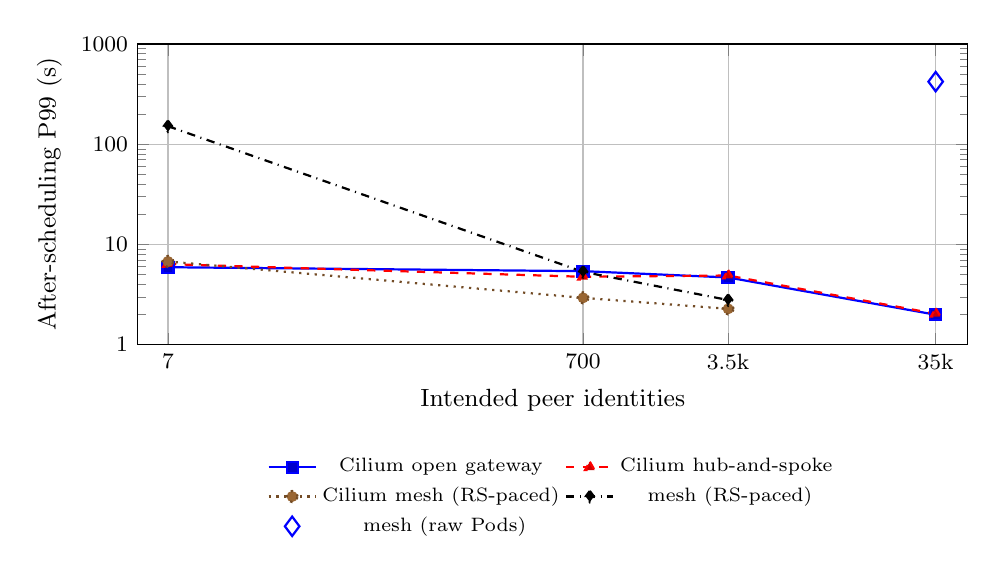
\begin{tikzpicture}
\begin{axis}[width=\linewidth,height=5.4cm,xmode=log,ymode=log,
	xmin=5,xmax=50000,ymin=1,ymax=1000,
	xtick={7,700,3500,35000},xticklabels={7,700,3.5k,35k},
	ytick={1,10,100,1000},yticklabels={1,10,100,1000},
	xlabel={Intended peer identities},ylabel={After-scheduling P99 (s)},
	tick label style={font=\footnotesize},label style={font=\small},
	legend style={font=\scriptsize,draw=none,at={(0.5,-0.34)},anchor=north,legend columns=2},
	grid=major]
\addplot+[mark=square*,thick] coordinates {(7,5.930) (700,5.416) (3500,4.685) (35000,1.990)};
\addlegendentry{Cilium open gateway}
\addplot+[mark=triangle*,dashed,thick] coordinates {(7,6.370) (700,4.759) (3500,4.899) (35000,2.033)};
\addlegendentry{Cilium hub-and-spoke}
\addplot+[mark=*,dotted,thick] coordinates {(7,6.767) (700,2.934) (3500,2.279)};
\addlegendentry{Cilium mesh (RS-paced)}
\addplot+[mark=diamond*,dashdotted,thick] coordinates {(7,151.479) (700,5.331) (3500,2.791)};
\addlegendentry{\sys{} mesh (RS-paced)}
\addplot+[only marks,mark=diamond,mark size=3.5pt,thick] coordinates {(35000,421.410)};
\addlegendentry{\sys{} mesh (raw Pods)}
\end{axis}
\end{tikzpicture}
\end{minipage}\hfill
\begin{minipage}{0.48\textwidth}
\centering
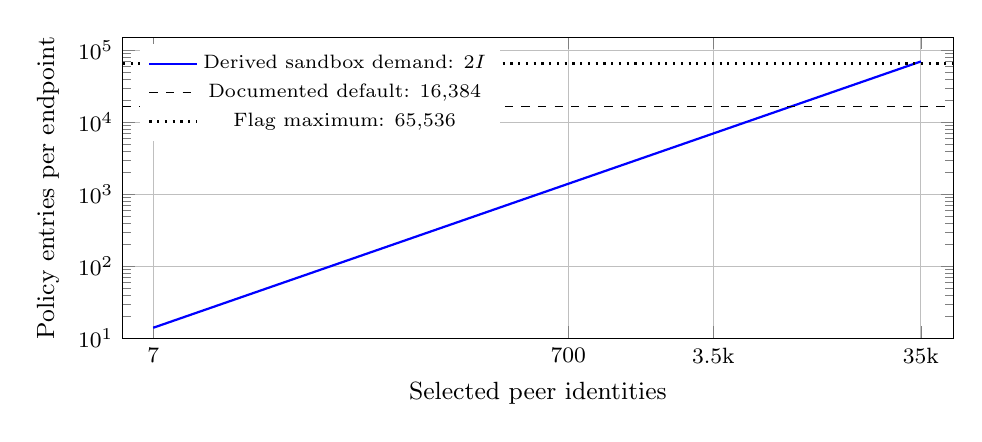
\begin{tikzpicture}
\begin{axis}[width=\linewidth,height=5.4cm,xmode=log,ymode=log,
	xmin=5,xmax=50000,ymin=10,ymax=150000,
	xtick={7,700,3500,35000},xticklabels={7,700,3.5k,35k},
	xlabel={Selected peer identities},ylabel={Policy entries per endpoint},
	tick label style={font=\footnotesize},label style={font=\small},
	legend style={font=\scriptsize,draw=none,at={(0.02,0.98)},anchor=north west},
	grid=major]
\addplot+[mark=none,thick] coordinates {(7,14) (700,1400) (3500,7000) (35000,70000)};
\addlegendentry{Derived sandbox demand: $2I$}
\addplot+[mark=none,dashed,black] coordinates {(5,16384) (50000,16384)};
\addlegendentry{Documented default: 16,384}
\addplot+[mark=none,dotted,black,thick] coordinates {(5,65536) (50000,65536)};
\addlegendentry{Flag maximum: 65,536}
\end{axis}
\end{tikzpicture}
\end{minipage}
\caption{Two meanings of scaling. Left: measured per-run after-scheduling
P99 on a logarithmic axis so that every executed tier is visible;
connecting lines are visual guides, each point is one run, and the
raw-Pod point has no matched Cilium run. Right: conditional
permission-state model for eager per-endpoint compilation
(Equation~\ref{eq:materialization} with $d=2$). The runner's header
records \texttt{--bpf-policy-map-max} as 65,536 on the Cilium cluster,
which admits the unidirectional 35k tiers and excludes the bidirectional
mesh at 35k ($2I=70{,}000 > 65{,}536$); the effective value was not
archived.}
\label{fig:scaling}
\end{figure*}

Within the ReplicaSet-paced tiers from 700 identities upward, neither
engine shows a rising post-scheduling tail. Cilium's open-gateway P99
falls from 5.930 s at 7 identities to 1.990 s at 35,000 (hub-and-spoke:
6.370 s to 2.033 s). In the mesh, \sys{} goes from 5.331 s P99 at 700
identities to 2.791 s at 3,500 (medians 3.273 s and 2.234 s), against
Cilium's 2.934 s and 2.279 s on the identical generator: within 2.4 s
and 0.5 s. Cilium's mesh medians are 1.412, 1.424, and 1.413 s across
its three tiers, so Cilium's typical Pod is faster than \sys{}'s at every
matched tier, and the tails converge only at 3,500 identities.

The two remaining \sys{} tiers are not flat, and they are why the figure
needs a log axis. At 7 identities with 5,000 Pods per ReplicaSet, \sys{}
recorded 38.946 s P50 and 151.479 s P99 after scheduling where Cilium
recorded 1.412 s and 6.767 s under the same configuration: a 22$\times$
P99 gap with zero JUnit failures on either side, and nothing in the
artifacts explains it. It is consistent with the July Kindnet baseline
(57.068 s P99) and tuned bundle (9.718 s after scheduling, 95.790 s
total) at the same 5,000-Pods-per-ReplicaSet shape, so the degradation
tracks large-ReplicaSet bursts rather than identity count.

The 35,000-identity \sys{} tier was run as 35,000 raw Pods under the mesh
policy and has no Cilium counterpart: the Cilium producer excluded the
mesh tier analytically (Section~\ref{sec:eval-capacity}), and Cilium's
only raw-Pod run used the hub-and-spoke policy and aborted
(Section~\ref{sec:eval-abort}). \sys{} completed it with all 35,000 Pods
Running and none stranded, at 120.003 s P50 / 421.410 s P99 after
scheduling and 139.557 s / 499.865 s end to end; the harness recorded
two JUnit failures against its 300-s P90 startup SLO (observed 357.7 s).
\texttt{create\_to\_schedule} alone reached 23.987 s P50 and 106.691 s
P99, so the scheduler was more than a minute behind for the tail before
any node did work. Candidate causes for the post-scheduling tail are
serialized sandbox creation in kubelet (about 49 Pods land on each
node), convergence of 35,000 new Pod addresses to the gateway nodes
before their init containers can be admitted, and API-server watch
latency; the kubelet CNI-latency query and all six \sys{} agent queries
returned no samples, so the artifacts do not separate them.

These results rule out the simple story that identity cardinality by
itself makes Cilium's admission collapse. They do not prove
identity-independent scaling for either engine, because the generator
changes controller fan-out and burst size with every tier:
Table~\ref{tab:resources} shows Cilium's achieved Phase-1 throughput at
277--328 Pods/s (median of per-second samples) in every tier with 10 or
more Pods per ReplicaSet and 169--170 Pods/s in the two
35,000-ReplicaSet tiers, with cluster-scoped Pod LIST P99 rising from
14--19 s to 28.8 s. The lowest Cilium tails coincide with a
controller-limited creation stream that halves the burst each node
absorbs.

The mesh tiers are the only place the two engines meet on the same
generator and policy, and two confounds still prevent reading them as an
engine comparison. First, the \sys{} runs created Pods at 124 and 103
Pods/s median against Cilium's 302 and 328 on the same configured 500
QPS and identical control-plane settings, so each \sys{} node absorbed
Pods at well under half the rate; by the argument just made that alone
lowers the tail, and the cause of the slower stream on the Kindnet
cluster is not recorded. Second, each cell is one trial. What the matched
tiers do support is narrower: under a generator Cilium handles at
2.3--2.9 s P99, \sys{} handles 700 and 3,500 identities at 2.8--5.3 s
P99 with the gateway-admission gate included, and its worker CPU does not
rise with identity count. Its end-to-end P99 at those tiers, 5.553 s and
2.918 s, is far below Cilium's 28.739 s and 21.730 s only because
\sys{}'s \texttt{create\_to\_schedule} P99 was 0.418 s and 0.231 s; that
component ends before any node or policy agent is involved.

\subsection{Resource and Control-Plane Measurements}
\label{sec:eval-resources}
Table~\ref{tab:resources} lists what the harness recovered about the
creation stream and the workers. Phase-1 throughput is the median and
P90 of per-second scheduled-Pod samples during the initial fill; CPU is
the September \texttt{instantaneous\_node\_cpu\_cores} query aggregated
across all 720 4-vCPU workers over the run.

\begin{table}[t]
\centering
\small
\setlength{\tabcolsep}{3pt}
\begin{tabular}{lrrrr}
\toprule
Scenario & Identities & \multicolumn{1}{c}{Pods/s} & \multicolumn{2}{c}{Node CPU (cores)}\\
 & & P50 / P90 & mean & P99\\
\midrule
Gateway & 7 & 284 / 377 & 0.52 & 0.71\\
 & 700 & 317 / 364 & 0.51 & 0.69\\
 & 3,500 & 316 / 372 & 0.54 & 0.69\\
 & 35,000 & 170 / 182 & 0.56 & 0.81\\
\midrule
Spoke & 7 & 0$^{\dagger}$ / 327 & 0.51 & 0.69\\
 & 700 & 323 / 398 & 0.61 & 0.86\\
 & 3,500 & 321 / 373 & 0.54 & 0.67\\
 & 35,000 & 169 / 181 & 0.55 & 0.78\\
\midrule
Cilium Mesh & 7 & 277 / 376 & 0.54 & 0.72\\
 & 700 & 302 / 351 & 0.54 & 0.67\\
 & 3,500 & 328 / 385 & 0.63 & 0.77\\
\midrule
\sys{} Mesh & 7 & 0$^{\dagger}$ / 310 & 0.52 & 0.66\\
 & 700 & 124 / 134 & 0.48 & 0.61\\
 & 3,500 & 103 / 106 & 0.45 & 0.56\\
 & 35,000 (Raw) & 0$^{\dagger}$ / 97$^{\ddagger}$ & 0.66 & 0.86\\
\midrule
Kindnet QPS 500 & $\sim$7 & 233 / 262 & 0.40 & 0.46\\
Kindnet tuned & $\sim$7 & 190 / 225 & 0.63 & 0.79\\
\bottomrule
\end{tabular}
\caption{Recovered Phase-1 scheduling throughput and worker-node CPU for
the runs in Tables~\ref{tab:identity} and~\ref{tab:qps}. CPU is the
harness's instantaneous node query on 4-vCPU workers, aggregated across
nodes over the run; the Kindnet QPS-500 row uses an earlier rate-based
query and is not directly comparable. $^{\dagger}$More than half of the
per-second samples were zero. $^{\ddagger}$Peak 841 Pods/s. No memory
series exists anywhere, and the six \sys{} agent queries added for the
mesh sweep (CPU, memory, packet processing time, verdict rate, queue
drops, user drops) returned \texttt{dataItems: null} in every tier
because the deployed Kindnet build exposes no metrics port.}
\label{tab:resources}
\end{table}

Worker CPU does not track intended identity count in either family.
Cilium's mean stays within 0.51--0.63 cores and its P99 within
0.67--0.86 across all eleven tiers and scenarios; \sys{} mesh stays
within 0.45--0.66 mean and 0.56--0.86 P99. The two \sys{} burst tiers
show single-node instantaneous maxima of 2.19 cores (tier 1) and 2.55
cores (tier 4), but the maximum of scrape-interval samples is not a
peak. All of this is a whole-node aggregate that includes kubelet,
containerd, and the sandbox workload itself; it cannot say what share the
policy agent took. It does exclude one thing: there is no CPU explosion
on the workers at 35,000 identities. If Cilium pays for identity
cardinality in these configurations, it pays in the operator, the API
server, or in map capacity, not in visible worker CPU. Cluster-scoped
Pod LIST P99 on the Kindnet cluster is 19.05, 8.24, 14.05, and 1.46 s
across the four mesh tiers, the last belonging to the raw-Pod tier whose
scheduler was 106 s behind, so API latency and scheduling backlog are
different symptoms. The \texttt{kindnetd} CPU term in the saved query has
no samples in any run, and every Cilium pprof capture requested through
the harness failed with connection refused; the $\lambda_q$, $\mu$, and
$M_{\mathrm{deferred}}$ terms of Section~\ref{sec:model} are unmeasured
here.

\subsection{Version Dependence}
\label{sec:eval-version}
Version matters as much as cardinality. An archived Cilium v1.18.6
attempt at the 700-identity gateway tier, run three hours before the
v1.20.1 sweep on the same day, retains only its generated configuration
and \path{cl2-metadata.json}; the harness never produced a startup
report. The repository's narrative records 34,981 Pods Running and 19
stranded in \texttt{Init:0/1} under default deny, and attributes the
outcome to a policy-cache race between identity allocation and endpoint
regeneration tracked as Cilium issue 7515 and fixed in
v1.20.0~\cite{cilium7515}. We have not reproduced that diagnosis, because
no logs from the attempt were kept. The narrower point stands on the
artifacts alone: the same generator at the same tier produced an
admission failure on one release and a clean 5.416-s P99 on the next.
\texttt{Init:0/1} is the state a sandbox stays in while
\texttt{wait-for-gateway} is still looping, so if the narrative's counts
are right, those 19 Pods are the one recorded instance of the enforcement
gate holding Pods back. Identity-scaling claims about
eager-materialization systems are release-specific, and a comparison has
to pin and report the version it ran.

\subsection{Capacity Exclusion Is Not a Latency Sample}
\label{sec:eval-capacity}
The mesh runner never attempted the 35,000-identity tier on Cilium. Its
\texttt{MESH\_SWEEPS} list is \texttt{(5000 50 10)}, omitting one Pod per
ReplicaSet, and it carries a guard that skips a listed tier when the
estimated per-endpoint entry demand reaches the configured map limit.
The model behind the guard assigns one entry per sandbox identity per
direction at every endpoint; Equation~\ref{eq:materialization} with
$d=2$ gives about 70,000 sandbox entries per endpoint at 35,000
identities, before gateway, DNS, or reserved-identity entries, which
exceeds the 65,536-entry value the runner documents. We call this an
\emph{analytical exclusion}: design evidence that a system can have low
latency throughout its feasible region and still hit a state-capacity
boundary. It is not evidence that an executed 35,000-identity mesh on
Cilium experienced insertion failures, packet loss, or any particular
latency, and it has no P99 to plot.

The effective \texttt{--bpf-policy-map-max} on the Cilium cluster is not
archived. In v1.20.1 source the flag defaults to 16,384 and is clamped to
at most 65,536~\cite{ciliumagentref}; the runner reads the value from the
\texttt{cilium-config} ConfigMap at run time, falls back to 16,384 if it
is unset, and its header comment records the tested value as 65,536. The
completed runs corroborate the higher value independently. The gateway
policy admits ingress from every sandbox identity, so at 35,000
identities each gateway endpoint needs about 35,000 entries; behind a
16,384-entry map, Pods past that count could not pass their
\texttt{wait-for-gateway} gate and would have stayed in
\texttt{Init:0/1}. All 35,000 reached \texttt{Running} in both
unidirectional 35,000-identity tiers with zero JUnit failures, so the
effective limit was at least 35,000 unless v1.20.1's identity aggregation
applied, and the source restricts aggregation to cluster-, world-, and
remote-node entity buckets rather than label selectors. One
\texttt{cilium-dbg bpf policy get} dump on a gateway node would have
settled the value; none was taken. The agent also offers an
endpoint-lockdown-on-overflow option~\cite{ciliumagentref}, so an
executed overflow would surface as denied traffic rather than as a
startup latency, one more reason the unrun tier has no P99.

Under the same model, 3,500 selected identities and 50 local endpoints
imply roughly 350,000 sandbox policy entries per node: derived demand,
not a map dump. The contrast with \sys{} is structural rather than
measured. Its design has no per-endpoint permission cross-product, so no
capacity guard excluded its 35,000-identity mesh tier, and that tier
completed with every Pod Running. Its limits sit in metadata storage,
conntrack sizing, and userspace verdict rate, and the 421-s tail of that
same tier is the reminder that removing the map bound does not by itself
make the tier cheap.

\subsection{An Aborted Direct-Burst Run}
\label{sec:eval-abort}
The raw-Pod microsegmentation record on the Cilium cluster documents a
different outcome. A run that created Pods directly, without
ReplicaSets, at the configured 500-QPS tier under the hub-and-spoke
policy aborted with 29,306 Running and 5,694 permanently stranded out of
35,000. The record attributes the abort to two mechanisms: concurrent
CNI ADD calls hitting the local Cilium REST API's HTTP 429 limit, and
cumulative identity allocation across creation and churn exhausting the
65,280 allocatable cluster-local identities, with the allocator
reporting ``no more available IDs in configured space.'' The harness
produced no final latency report, so the run appears in
Table~\ref{tab:identity} as a completion count and nothing else.

A missing percentile file is not a reason to drop a failed run, nor to
promote the documented diagnosis to a reconstructed timeline. Allocator
history, identity garbage-collection behavior, effective limiter
settings, and the agent logs would be needed to separate the two causes
and order them; none were retained. The identity allocator is
cluster-level state, distinct from the per-endpoint policy-map capacity
of Section~\ref{sec:eval-capacity}; 65,280 and 65,536 are different
limits on different structures. And a direct Pod burst is a different
workload from ReplicaSet-mediated creation, which is why this run and the
\sys{} raw-Pod mesh tier are separated in Table~\ref{tab:identity}
rather than compared. The abort supports an admission-failure case
study, not a claim that every 35,000-identity workload fails on Cilium.

\subsection{Connection Cost and Correctness}
\label{sec:eval-connection}
The collection measures workload admission and the control-plane
activity around it, not the core packet-admission tradeoff of
Section~\ref{sec:design}: NFQUEUE verdict capacity, established-flow
throughput parity, and isolation through startup and failure are all
unmeasured. Because the \texttt{wait-for-gateway} gate folds one admitted
connection into every \texttt{schedule\_to\_run} sample, the sweeps do
bound first-permitted-connection latency on one path, but they cannot
isolate that component from image pull and container start, a configured
mesh permission does not generate all-to-all traffic, and reaching
\texttt{Running} tests no forbidden peer relationship. The only negative
check is the one-shot smoke test of Section~\ref{sec:eval-method}.

The only connection-level data point anywhere is the implementation
repository's own three-node microbenchmark summarized in
Section~\ref{sec:model}: 10,000 non-keepalive HTTP requests at
concurrency 1,000 completed at 2,317 requests/s through the queue with a
5-ms median and a 3,080-ms P99 while the kernel logged
\texttt{nf\_conntrack: table full} at 262,144 entries, with per-node
queued-packet peaks near 8,000 packets/s and callback medians of
80--120 $\mu$s~\cite{knptesting}. It dates from April 2024 and records no
hardware, kernel, or agent version, so we treat it as indicative. Read
against the sweeps, it says that a node absorbing about 50 sandboxes
while the cluster creates 103--328 Pods/s is nowhere near the queue's
connection limit, and that on that node the limit was reached first by
conntrack capacity, not by the userspace evaluator. It does not say what
happens under sustained denied traffic, whether the 3-s P99 is queueing
or conntrack, or how either changes with policy count. Nothing in the
cluster artifacts exercises the IPTracker flavor of
Section~\ref{sec:iptracker}, whose divert-all steering would give the
same workload a different $\lambda_q$. The discriminating experiments,
and the order in which they should be run, are in
Section~\ref{sec:discussion}; the first of them is a single-node
connection microbenchmark with a denied-traffic mix, run into overload
in both overflow modes, to locate the capacity boundary of
Section~\ref{sec:design}.

\subsection{Control-Plane Sensitivity}
\label{sec:eval-qps}
The July QPS sweeps are why startup has to be decomposed at all.
Table~\ref{tab:qps} reports the primary saved Cilium and Kindnet baseline
runs. At QPS 500 the after-scheduling P99s are 5.482 s and 57.068 s
(medians 1.490 s and 7.922 s), so the archived baseline does not
establish any startup advantage for the NFQUEUE-based configuration; at
the burst shape the July runs used it shows the opposite. At QPS 50 and
100 both families record two JUnit failures. All four are the same
measurement, \texttt{WaitForOldPodsDeleted-Final}, timing out while 5,024
to 19,999 churned sandbox Pods were still terminating. No startup-phase
measurement failed, so the startup percentiles in those rows are
complete, but the runs did not finish teardown within the harness
deadline, and Pod deletion latency at those tiers is unmeasured.

\begin{table}[t]
\centering
\small
\begin{tabular}{rrrrr}
\toprule
QPS & \multicolumn{2}{c}{After scheduling P99} & \multicolumn{2}{c}{Total P99}\\
tier & Cilium & Kindnet & Cilium & Kindnet\\
\midrule
$50^{*}$ & 4.065 & 4.833 & 4.089 & 4.855\\
$100^{*}$ & 1.788 & 7.143 & 1.814 & 7.378\\
200 & 1.845 & 59.347 & 2.285 & 59.485\\
500 & 5.482 & 57.068 & 11.160 & 57.629\\
\bottomrule
\end{tabular}
\caption{Archived primary QPS runs, July 2026; all values in seconds.
Asterisks mark tiers whose only JUnit failures are final-teardown
deletion timeouts in both configurations; startup measurements
completed. These are complete-stack observations on two clusters, not an
isolated NFQUEUE-versus-eBPF comparison.}
\label{tab:qps}
\end{table}

The Kindnet cluster was then tuned in five steps that changed the agent
version, the NRI socket mount, and API Priority and Fairness (APF)
settings together. The final bundle, labeled v1.0.1 with NRI and an APF
exemption, records an after-scheduling P50 of 2.345 s and P99 of 9.718 s.
Its total P99 is nevertheless 95.790 s, with a create-to-schedule P99 of
94.555 s: the tail moved from the node to the scheduler. That is direct
evidence against reading a reduced post-scheduling tail as an end-to-end
speedup, and because the variables changed together the sequence is a
tuning chronology, not an NRI ablation. A separate Cilium QPS-500
repetition records 4.257 s after scheduling and 12.404 s total; it is
kept as a second trial beside the 5.482 s and 11.160 s primary, not
averaged with it. The recovered throughput rows add one more caution: the
verified Cilium QPS-500 run achieved 180/412 Pods/s P50/P90 while the
Kindnet baseline achieved 233/262 and the tuned bundle 190/225, so at
this tier the Kindnet cluster's median creation rate was higher than the
Cilium cluster's when its tail was worst, the reverse of the mesh-tier
confound.

APF divides API-server concurrency among request classes and provides
queueing and isolation between them~\cite{k8sapf}. Exempting a class or
raising its share moves contention to other classes; it does not create
capacity. The wider limitations apply to everything above: most
configurations have one trial, summary percentiles hide time variation
and preclude per-Pod trajectories, failed JUnit elements are not failed
Pods, and instantaneous CPU maxima at the scrape interval are not peaks.

\subsection{What the Artifacts Still Do Not Contain}
\label{sec:gaps}
The \sys{} mesh sweep closes the largest gap of the earlier draft: a
\sys{} run above seven identities now exists at 700, 3,500, and 35,000.
It does not close the comparison. The six \sys{} agent queries and the
kubelet CNI-latency query added for that sweep returned no samples in
all four tiers, and the repository's own probe script concludes that the
deployed Kindnet build has the agent metrics endpoint disabled.
Table~\ref{tab:gaps} lists what remains: the missing evidence, the claim
it would support or refute, and the cheapest experiment that would
produce it.

\begin{table}[t]
\centering
\footnotesize
\setlength{\tabcolsep}{4pt}
\begin{tabular}{R{2.35cm}R{2.15cm}R{2.85cm}}
\toprule
Missing evidence & Claim at stake & Cheapest producer\\
\midrule
Agent CPU, memory, verdict rate, latency, drops (all six queries empty) & where displaced work lands; $\lambda_q$, $\mu$, overflow margin & rebuild Kindnet with the metrics server enabled; rerun one tier\\
\addlinespace
Cause of the \sys{} 151 s and 421 s tails & burst behavior of the \sys{} node path & collect init-container \texttt{Latency:} logs and kubelet PLEG/CNI metrics on a sample of nodes\\
\addlinespace
Why \sys{} runs created Pods at 103--124 Pods/s versus Cilium's 302--328 & validity of the matched-tier comparison & compare controller-manager and API-server metrics of the two clusters\\
\addlinespace
A Cilium raw-Pod mesh run or a \sys{} 1-Pod-per-ReplicaSet 35k run & a matched pair at 35,000 identities & one additional run on either cluster\\
\addlinespace
Repeat trials & any statistical statement & rerun tiers 2--3 on both clusters\\
\addlinespace
Policy-map occupancy dump and the effective map-size flag & capacity model of Fig.~\ref{fig:scaling} & \texttt{cilium-dbg bpf policy get} and the ConfigMap on one node\\
\addlinespace
Denied traffic under load & isolation, deny amplification & single-node connection microbenchmark with deny mix, both overflow modes\\
\addlinespace
NRI on/off with identical binaries & startup-metadata benefit & rerun baseline QPS 500 and tuning bundle 1 with one pinned image\\
\addlinespace
Binary digests and flags per run; logs for both aborts & attribution and causal diagnosis & record in \texttt{cl2-metadata}; retain logs on abort\\
\bottomrule
\end{tabular}
\caption{Evidence still absent from the benchmark and implementation
repositories after the \sys{} mesh sweep.}
\label{tab:gaps}
\end{table}

Two absences are cheap to fix: the per-Pod \texttt{Latency: N ms} lines
that every init container already prints would, if scraped, split the
gate from container start in every sample, and archiving
\path{scripts/verify-netpol.sh} output per run instead of once per
cluster costs seconds. Until both are done, the enforcement claim rests
on a per-Pod positive gate and a single unarchived negative check.
